%\section{Ziel}
%\label{sec:Ziel}
%Das Ziel dieses Versuchs ist es, bestimmte Eigenschaften eines Helium-Neon-Lasers zu bestimmen.
%Dazu zählen die Wellenlänge, einige Moden und die Polarisation.

\section{Theorie}
\label{sec:Theorie}

\subsection{Aufbau und Prinzip eines Lasers}
%3 Komponenten
Ein Laser (light amplification by stimulated emission of radiation) besteht aus drei Komponenten: einer Energiepumpe, einem verstärkenden Medium und einem Resonator.
Durch die Energiepumpe wird dem verstärkenden Medium Energie zugeführt, was zu induzierter Emission durch die aktivierten Atome des Mediums führt. Der Resonator schickt das emittierte Licht durch optische Rückkopplung wieder durch das verstärkende Medium. Ein Laser ist also ein optischer Oszillator. \cite{Laserspektroskopie}

%Wellenlänge
Die Wellenlänge eines Lasers wird durch den Übergang zwischen zwei Energieniveaus des aktiven Mediums definiert. Die Atome gehen dabei unter Abgabe eines Photons
der Frequenz
\begin{equation*}
    \nu = \frac{E_\text{k} - E_\text{i}}{h}
    %\label{eq:nu}
\end{equation*}
vom angeregten Zustand $E_\text{k}$ in den tieferen Zustand $E_\text{i}$ über. \cite{Laserspektroskopie}


%\subsection{Aktives Medium}
%Prozesse
%Im aktiven Medium treten folgende Prozesse auf:
%\begin{itemize}
%    \item induzierte Absorption: ein Photon wird absorbiert und regt dabei das Atom vom Zustand $E_1$ in den energetisch höheren Zustand $E_2$ an. Dabei gilt die Bedingung \eqref{eq:nu}.
%    \item induzierte Emission: ein Atom im angeregten Zustand $E_2$ wird durch ein äußeres Strahlungsfeld (einfallendes Photon) dazu veranlasst, unter Emission eines zweiten Photons mit Frequenz \eqref{eq:nu} in den tieferen Zustand $E_1$ überzugehen. Das zweite Photon besitzt die gleichen optischen Eigenschaften wie das einfallende.
%    \item spontane Emission: ein angeregtes Atom gibt ohne den Einfluss eines äußeren Feldes seine Anregungsenergie unter Emission eines Photons ab.
%\end{itemize}

%Inversion
%Die Verstärkung eines Strahls durch induzierte Emission kann nur stattfinden, wenn Besetzungsinversion zwischen dem Grundzustand und dem Laserniveau herrscht. Das bedeutet, dass die Besetzungsdichte des Laserniveaus höher wird als die Besetzungsdichte des energetisch tiefer liegenden Niveaus (Zustand, in dem sich mehr Atome in einem höheren Energieniveau befinden als im tieferen). Dadurch ist die induzierte Emissionsrate größer als die Absorptionsrate und Licht kann beim Durchgang durch das aktive Medium verstärkt werden.


%beim He-Ne-Laser
Das aktive Medium beim He-Ne-Laser ist ein Helium-Neon-Gasgemisch. Diesem wird in einer elektrischen Entladung Energie zugeführt. Die durch die Ionisation gelösten Elektronen stoßen mit den He-Atomen, die dadurch in einen angeregten Zustand versetzt werden. Die Energie dieser angeregten He-Atome wird durch sogenannte Stöße zweiter Art auf die Ne-Atome übertragen. Die He-Atome wirken also als Energiepumpe für die Ne-Atome. Die nun angeregten Ne-Atome gehen unter Emission eines Photons in ein tiefer liegendes Niveau über. Dieser Übergang definiert, wie zuvor beschrieben, die Wellenlänge das Lasers. \cite{Laser}



%\subsection{Pumpschemen}
Es gibt Drei-Niveau- und Vier-Niveau-Laser.
Bei Vier-Niveau-Lasern ist $E_3$ das obere Laserniveau, welches langlebig ist. Das kurzlebige Niveau $E_4$ steht für alle darüberliegenden Niveaus. Das untere Laserniveau $E_2$ ist ebenfalls kurzlebig. Das Grundniveau wird durch $E_1$ beschrieben.
Beim Drei-Niveau-Laser ist das Grundniveau $E_1$ auch das untere Laserniveau. \cite{Photonik}
%Dadurch sind diese Laser ineffizienter als Vier-Niveau-Laser, da ... keine Ahnung.

%Zwei-Niveau-Laser sind nicht möglich, da ... ?

Beim He-Ne-Laser handelt es sich um einen Vier-Niveau-Laser.
Der Übergang von $3s_2$ nach $2p_4$ ist für die rote Linie verantwortlich. \cite{Laser}

%Wie wird der Besetzungsinversion erreicht?

%\subsection{Bestimmung der Wellenlänge}
%Formel

Die Wellenlänge eines Lasers lässt sich mithilfe eines Gitters mit der Formel 
\begin{equation}
    \lambda = \frac{b \cdot a}{\sqrt{d^2 + a^2}}
    \label{eq:welle}
\end{equation}
bestimmen, wobei $b$ der Spaltbreite des Gitters entspricht, $a$ dem Abstand der Maxima und $d$ der Entfernung zwischen Gitter und Schirm.

\subsection{Optischer Resonator und Stabilität}
%Stabilitätsparameter
Bei einem optischen Resonator verteilt sich das Strahlungsfeld nicht auf alle Moden, sondern bleibt auf wenige konzentriert. Für diese Moden hat der Resonator kleine Verlustfaktoren, für den Rest große. Die Wahrscheinlichkeit der induzierten Emission wird in den verlustarmen Moden größer, wodurch die Pumpenergie bevorzugt in Strahlungsenergie dieser Moden umgesetzt wird. \cite{Laserspektroskopie}

In einem stabilen Resonator reproduziert sich die Feldverteilung nach jedem Umlauf der Welle.
Die Stabilitätsbedingung lautet
\begin{equation}
    0 < g_1 \cdot g_2 < 1 \text{ oder } g_1 = g_2 = 0,
    \label{eq:stabilitaet}
\end{equation}
wobei $g_\text{i}$ die Stabilitätsparameter sind.
Für diese gilt
\begin{equation}
    g_1 \cdot g_2 = \left(1-\frac{d}{b_1} \right)\cdot\left(1-\frac{d}{b_2} \right),
    \label{eq:parameter}
\end{equation}

wobei d die Länge des Resonators, also der Abstand der Spiegel, und $b_\text{i}$ jeweils der Krümmungsradius des Spiegels ist. \cite{Laserspektroskopie}

Die Stabilitätsparameter für zwei verschiedene Resonatoren sind in den Abbildungen \ref{fig:stability1} und \ref{fig:stability2} mithilfe von Formel \ref{eq:parameter} dargestellt.

\begin{figure}
    \centering
    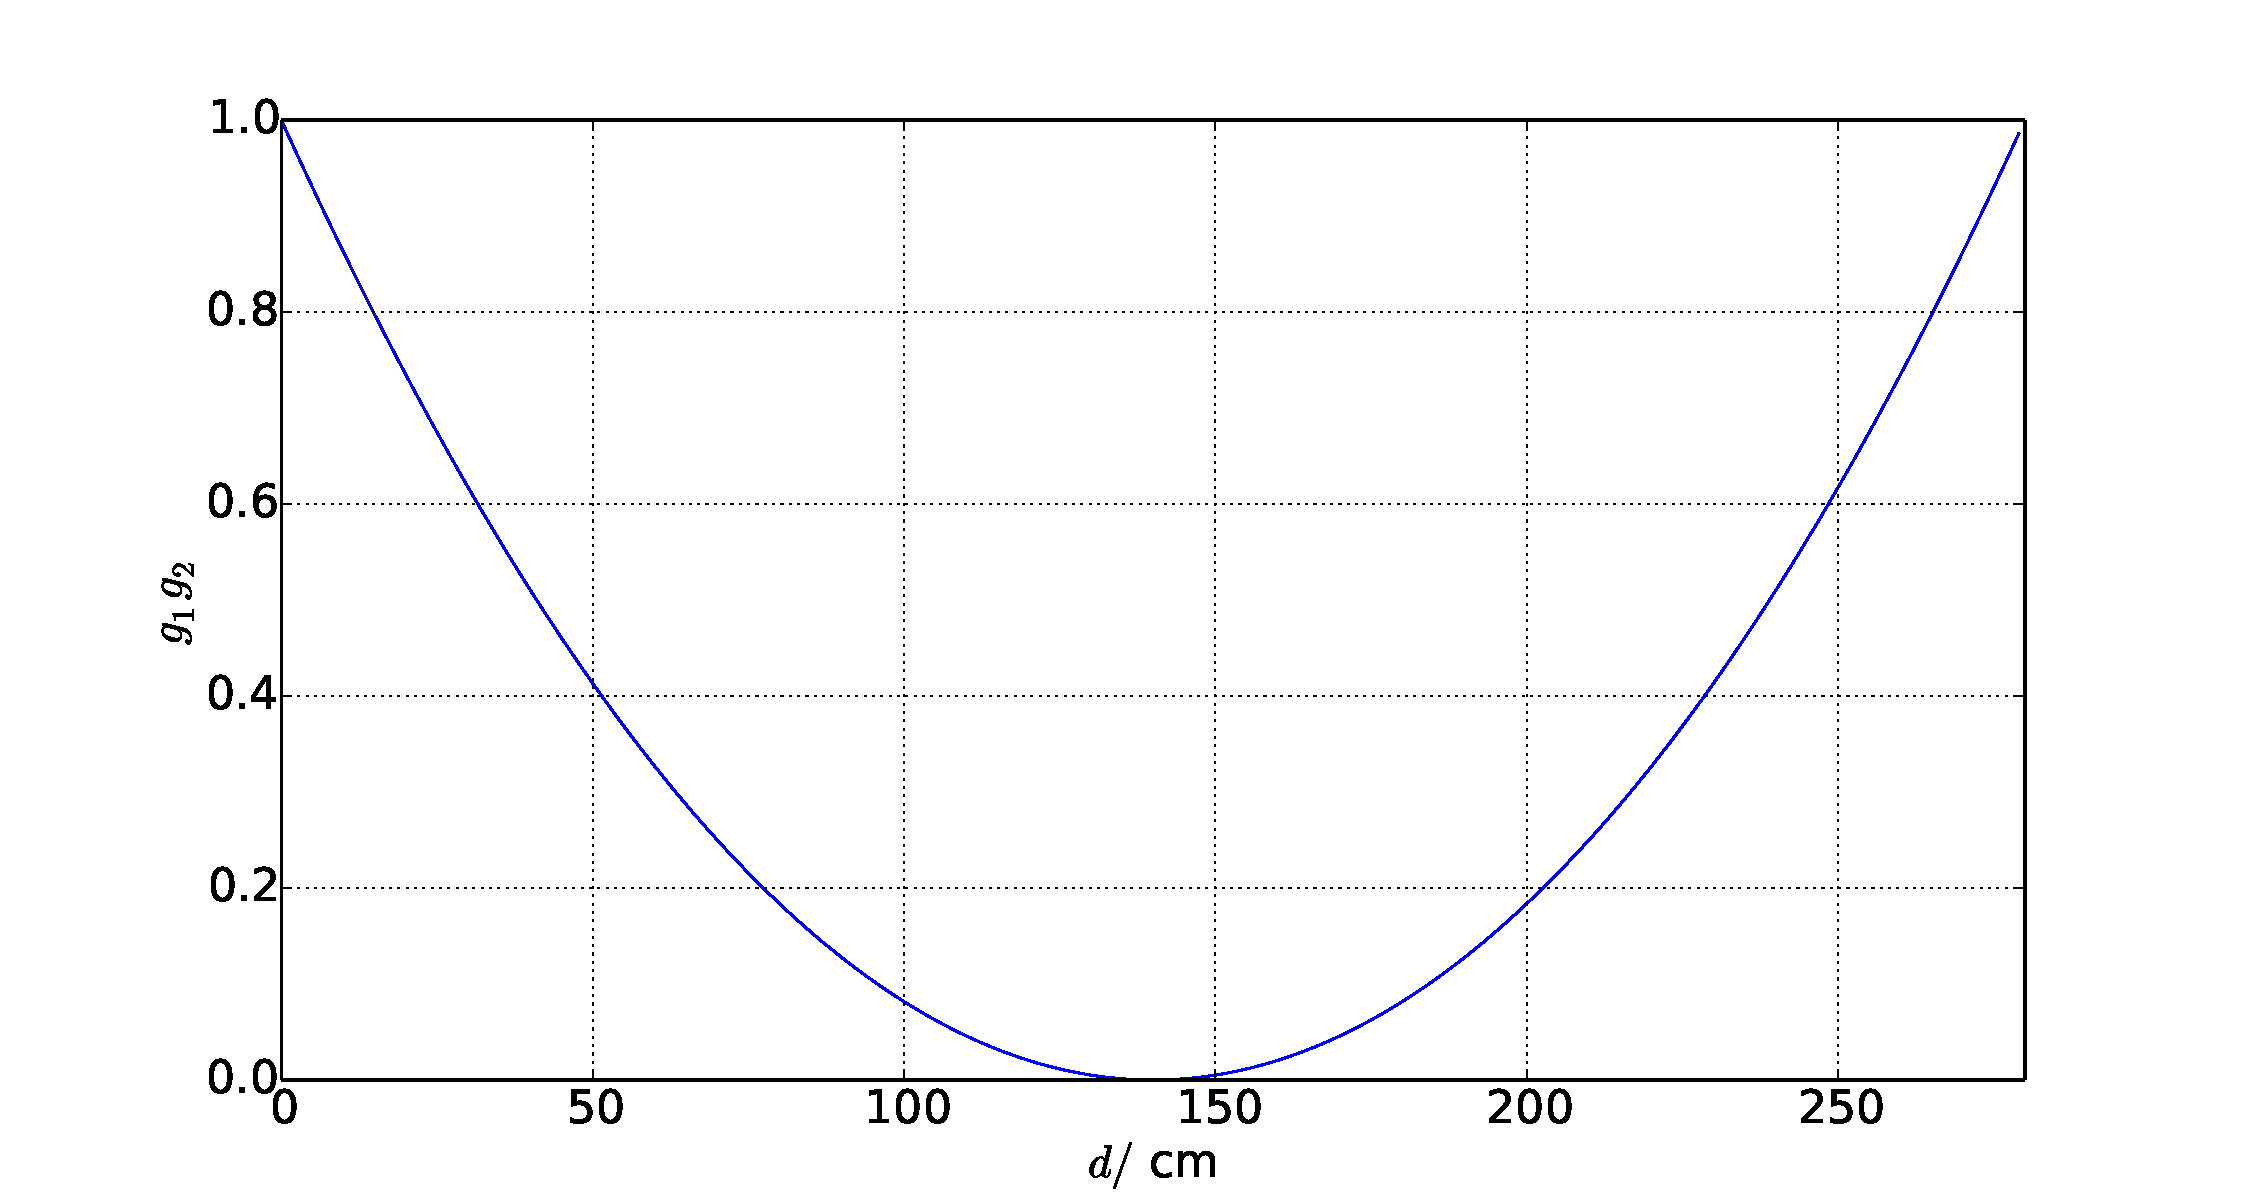
\includegraphics[width=0.8\textwidth]{plots/stability1.pdf}
    \caption{Die Stabilitätsparameter für zwei konkave Spiegel mit jeweils einem Krümmungsradius von $b_\text{i} = \SI{140}{\centi\meter}$ sind in Abhängigkeit von der Resonatorlänge dargestellt. Der maximale Resonatorabstand beträgt $d = \SI{280}{\centi\meter}$.}
    \label{fig:stability1}
\end{figure}

\begin{figure}
    \centering
    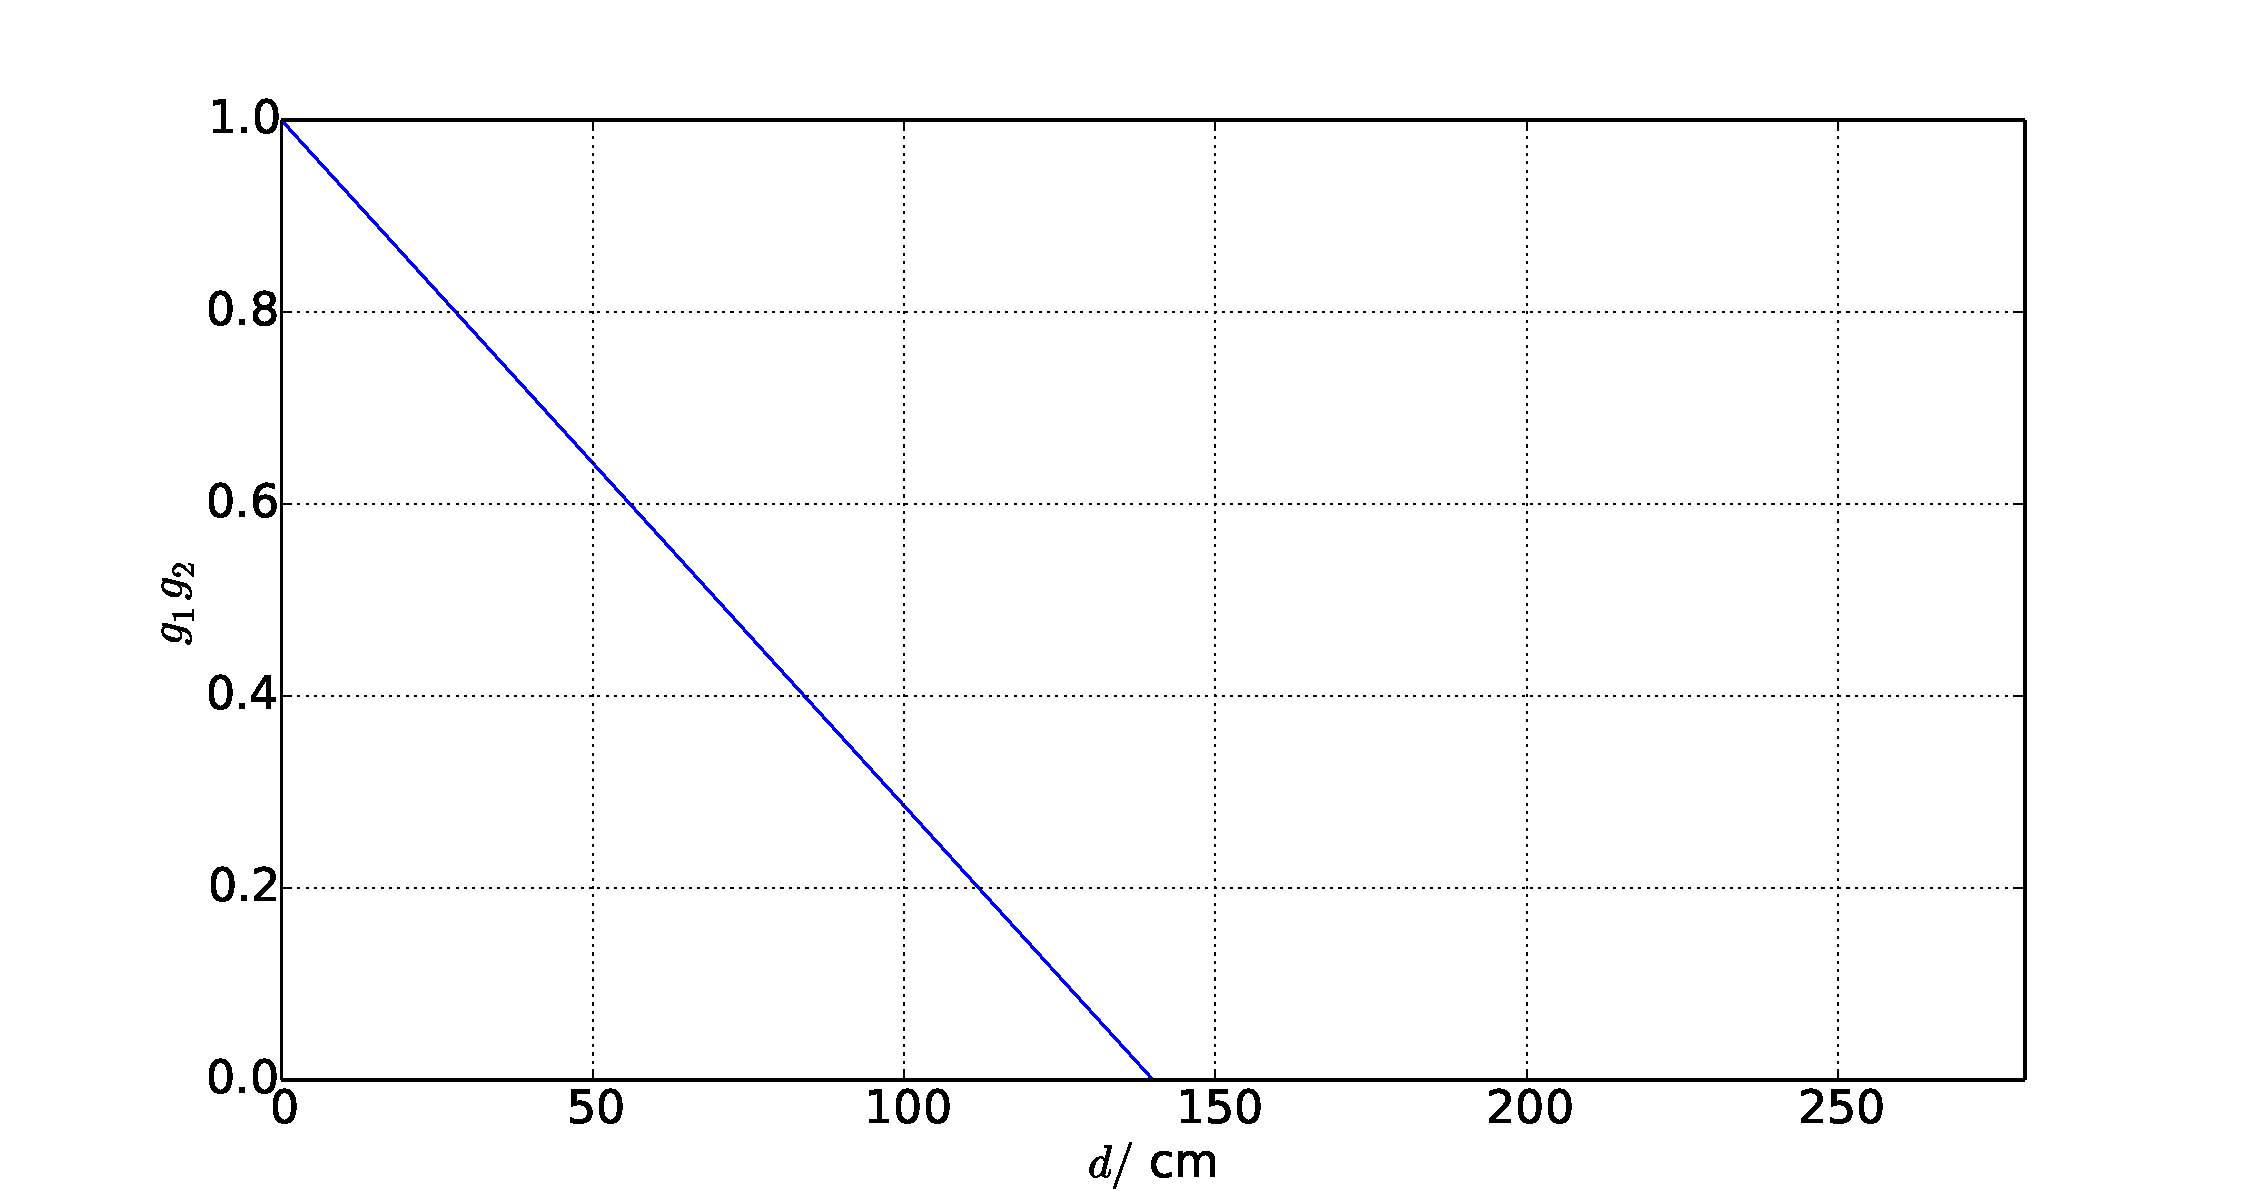
\includegraphics[width=0.8\textwidth]{plots/stability2.pdf}
    \caption{Die Stabilitätsparameter für einen flachen und einen konkaven Spiegel mit einem Krümmungsradius von $b_2 = \SI{140}{\centi\meter}$ sind in Abhängigkeit von der Resonatorlänge dargestellt. Der maximale Resonatorabstand beträgt $d = \SI{140}{\centi\meter}$.}
    \label{fig:stability2}
\end{figure}

\subsection{Moden im Resonator}
\label{sec:model}
%TEM$_{mn}$ Moden sind stationäre Feldverteilungen.
%Die TEM$_{00}$-Mode heißt Fundamental- bzw. axiale Mode.
%Die Fundamentalmoden haben ein radial-symmetrisches Gauß’sches Intensitätsprofil. Senkrecht zur Resonatorachse sinkt die Intensität auf $1/e^2$ ihres Wertes $I_0$ auf der Achse. Man nennt w den Radius der TEM$_{00}$-Mode. Der minimale Radius $w_0$ liegt bei $z=0$, d. h. in der Mitte des konfokalen Resonators.
%Der Parameter $w_0$ heißt die Strahltaille der Resonatormode.

%Modenblende:
Zur Selektion einzelner TEM$_{mn}-$Moden eines Multimodenlasers können optische Elemente in den Resonator eingesetzt werden, welche die Oszillation der unerwünschten Moden (höhere Moden) unterdrücken.
%Transversale Moden (TEM-Moden) sind elektromagnetische Eigenschwingungszustände eines Systems in transversaler Richtung, also senkrecht zur Ausbreitungsrichtung.
%Longitudinal Moden laufen längs der Ausbreitungsrichtung. 
%Die Anzahl der longitudinalen Moden gibt Aufschluss über die Anzahl der Wellen, die im Resonator schwingen können.
%Für deren Auswahl eignet sich ein Fabry-Pérot-Interferometer.

Die Amplitudenverteilung der TEM-Moden kann mit der Formel 
\begin{equation}
    A_{m,n}\left(x,y,z\right) = C_{mn} H_m\left(x^*\right)\cdot H_n\left(y^*\right) \cdot \exp\left(-\left( x^{*2} + y^{*2} \right)/4 \right) \exp\left( -i \phi \left( x,y,z \right)\right) 
    \label{eq:amp}
\end{equation}
beschrieben werden, wobei $C_{mn}$ ein Normierungsfaktor ist, $H_m$ und $H_n$ die Hermiteschen Polynome darstellen und $x^*$ und $y^*$ die normierten Koordinaten mit $x^*= \sqrt{2} x/w$ und  $y^*= \sqrt{2} y/w$ sind mit 
\begin{equation*}
    w(z) = \sqrt{\lambda \cdot \frac{d}{2\pi}\left[ 1 + \left(\frac{2z}{d} \right)^2 \right]},
\end{equation*}
wobei $\lambda$ die Wellenlänge und $d$ die Resonatorlänge ist. Für die Intensitätsverteilung gilt $I\left(x,y\right) \propto \absolutevalue{A_{mn}}^2$. \cite{Laserspektroskopie}

Daraus ergibt sich mit Formel \eqref{eq:amp} für die 
TEM$_{00}$-Mode der Ausdruck 
\begin{equation}
    I(x,y) = I_0 \cdot \frac{2}{w^2} \cdot \exp\left(-\left(\frac{(x - \mu)}{w}\right)^2\right).
    \label{eq:mode0}
\end{equation}
Für die TEM$_{10}$-Mode und die TEM$_{20}$-Mode gilt dies analog.



% \subsection{Multimode- und Singlemode-Laserbetrieb}

% Singlemode sind schmalbandig.
% Man unterscheidet Single-Mode-Laser, die nahezu auf nur einer Frequenz schwingen, und Multimode-Laser, welche mehrere Farblinien emittieren. 

% %Doppler-Effekt
% Eine Form der inhomogenen Linienverbreiterung ist die Dopplerverbreiterung in Gasen. Die Frequenz eines Photons ist abhängig von der Geschwindigkeit des emittierenden Atoms relativ zur Beobachtungsrichtung. Die Linienform ergibt sich als Überlagerung mehrerer Beiträge, also durch die unterschiedlichen Ausbreitungsrichtungen der Gasmoleküle.
% (etwas wenig)


%Verbreitung für den Neon-Übergang

%Modenspektrum für Laser mit L=1,5m
% %Fabry-Pérot-Etalon
% Modenselektion mithilfe des Fabry-Pérot-Etalon:
% Das Fabry-Pérot-Etalon ist ein optischer Resonator, der aus zwei teildurchlässigen Spiegeln in unveränderlichem Abstand besteht. Eintreffendes Licht wird nur transmittiert, wenn die Wellenlängen die Resonanzbedingung des Resonators erfüllen.
% Andere Bereiche werden durch destruktive Interferenz der Teilstrahlen fast vollständig ausgelöscht. 


\subsection{Polarisation eines Lasers}
%Brewster-Fenster
Durch Einfügen eines Brewster-Fensters in den Resonator kann eine Polarisationsrichtung selektiert werden.
Die Fensterflächen stehen  zur optischen Achse im Brewster-Winkel. Licht, das unter dem Brewster-Winkel auftrifft und parallel zur Einfallsebene polarisiert ist, wird an der Oberfläche nicht reflektiert, sondern tritt ohne Verlust durch das Brewster-Fenster. Die senkrecht zur Einfallsebene polarisierte Komponente des Lichts wird allerdings reflektiert und somit im Laser unterdrückt.

Das Model, mit dem sich die Polarisation beschreiben lässt, lautet 

\begin{equation}
    P(\phi) = P_0 \cdot \cos\left( \phi + \delta \right)^2. 
    \label{eq:polar}
\end{equation}
%resultierende Polarisation